\documentclass[portrait,final,a0paper,fontscale=0.284]{baposter}

\usepackage[utf8]{inputenc}
\usepackage[T1]{fontenc}
\usepackage[provide=*,spanish]{babel}
\usepackage{graphicx}
\usepackage{amsmath}
\usepackage{booktabs}
\usepackage{colortbl}
\usepackage{tabularx}
\usepackage{multicol}
\usepackage{url}
\usepackage{tikz}
\usetikzlibrary{arrows.meta,calc,positioning,shapes.geometric}

\graphicspath{{images/}}

% Paleta institucional sobria y de alto contraste.
\definecolor{navy}{RGB}{18,53,84}
\definecolor{blue}{RGB}{25,116,168}
\definecolor{cyan}{RGB}{35,166,189}
\definecolor{pale}{RGB}{235,246,249}
\definecolor{orange}{RGB}{231,111,41}
\definecolor{ink}{RGB}{35,43,49}
\definecolor{muted}{RGB}{91,105,116}
\definecolor{good}{RGB}{34,139,94}

\newcommand{\compresslist}{%
  \setlength{\itemsep}{2pt}%
  \setlength{\parskip}{0pt}%
  \setlength{\parsep}{0pt}%
}

\newcommand{\keynumber}[3]{%
  \begin{tikzpicture}[baseline=(n.base)]
    \node[draw=#1!75!black,fill=#1!10,rounded corners=4pt,
      inner xsep=0.65em,inner ysep=0.42em,text width=0.88\linewidth,
      align=center] (n) {\textcolor{#1!75!black}{\LARGE\bfseries #2}\\[-0.15em]
      \small\textcolor{ink}{#3}};
  \end{tikzpicture}%
}

\begin{document}

\begin{poster}
  {
    grid=false,
    columns=3,
    colspacing=0.9em,
    bgColorOne=white,
    bgColorTwo=white,
    borderColor=blue,
    headerColorOne=navy,
    headerColorTwo=blue,
    headerFontColor=white,
    boxColorOne=white,
    boxColorTwo=pale,
    textborder=roundedleft,
    eyecatcher=true,
    headerborder=closed,
    headerheight=0.112\textheight,
    headershape=roundedright,
    headershade=shadelr,
    headerfont=\Large\bfseries\scshape,
    textfont={\color{ink}\raggedright\setlength{\parindent}{0em}\setlength{\parskip}{0.42em}},
    boxshade=plain,
    background=plain,
    linewidth=1.8pt
  }
  {
\includegraphics[height=6.5em]{logo_uni.png}}
  {\Large\bfseries\scshape Extracción automática de resultados electorales\\
   a partir de actas de escrutinio de las Elecciones Generales del Perú 2026}
  {\normalsize Josemanuel Rossy Cañari Palante, Kenny Asto Hinostroza,\\
   Melissa Dessire Aylas Barranca y Carlos Pérez Pérez\\[0.25em]
   \small Maestría en Inteligencia Artificial - Visión por Computador, Grupo 3\\
   Universidad Nacional de Ingeniería, Lima, Perú}
  {}

% -----------------------------------------------------------------------------
% COLUMNA IZQUIERDA
% -----------------------------------------------------------------------------
\headerbox{Problema y objetivo}{name=problem,column=0,row=0}{
  Muchas actas de escrutinio se publican como formularios escaneados con conteos
  manuscritos. Revisar aproximadamente \textbf{88,064 mesas} no es escalable y
  limita la auditoría automática.

  \textbf{Objetivo.} Evaluar la precisión de un sistema reproducible de visión
  por computador para extraer resultados y definir los requisitos de una
  solución de uso real.
}

\headerbox{Diseño del estudio}{name=design,column=0,below=problem}{
  \begin{itemize}\compresslist
    \item \textbf{Fuente y muestra:} portal ONPE, primera vuelta del 12 de abril
      de 2026; muestreo aleatorio simple con semilla pública 2026:
      \textbf{100 actas de 23 departamentos}.
    \item \textbf{Tipos documentales:} 76 actas manuscritas escaneadas y 24 actas
      digitales STAE con capa de texto.
    \item \textbf{Referencia:} conteos digitados y publicados por la ONPE; no se
      requirió etiquetado manual.
    \item \textbf{Unidad de evaluación:} 43 campos por acta manuscrita, luego de
      excluir las posiciones 04 y 14 de partidos retirados; \textbf{3,268 campos}
      en total.
  \end{itemize}
}

\headerbox{Evaluación}{name=evaluation,column=0,below=design}{
  La \textbf{exactitud por campo} mide coincidencia exacta con el valor oficial;
  el \textbf{CER} cuantifica las ediciones de caracteres y debe minimizarse.
  Los IC del 95\% se estimaron con \textbf{10,000 remuestreos de actas
  completas}, preservando la dependencia intradocumento.
}

\headerbox{Alcance e interpretación}{name=scope,column=0,below=evaluation}{
  \begin{itemize}\compresslist
    \item La muestra evalúa desempeño, pero no estima con precisión la proporción
      poblacional de actas STAE.
    \item La regla ``celda vacía = 0'' incorpora conocimiento del formulario y
      se reporta separada del reconocimiento estrictamente visual.
    \item El desempeño alcanzado en manuscritos aún exige validación humana; el
      sistema constituye una línea base especializada, no una automatización
      electoral autónoma.
  \end{itemize}
}

\headerbox{Código y referencias}{name=references,column=0,below=scope}{
  \small Repositorio: \texttt{github.com/carlosperez100/}\\[-0.2em]
  \texttt{onpe\_actas}

  Referencias: Zhao et al. (CVPR 2024); Fujitake (WACV 2024); Wan et al.
  (CVPR 2024); Li et al. (AAAI 2023); Kim et al. (ECCV 2022).
}

% -----------------------------------------------------------------------------
% DOS COLUMNAS DERECHAS
% -----------------------------------------------------------------------------
\headerbox{Sistema propuesto}{name=system,column=1,span=2,row=0}{
  \begin{center}
  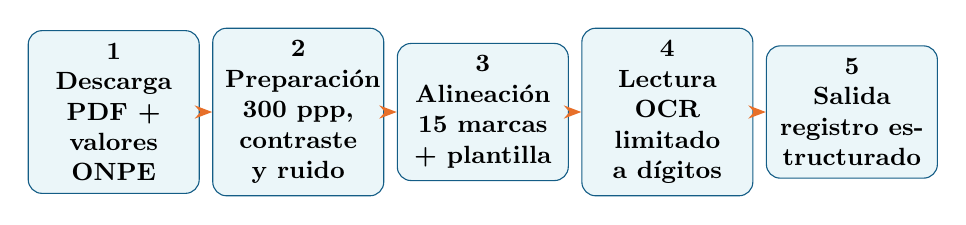
\begin{tikzpicture}[
    node distance=0.45em,
    flowbox/.style={draw=blue!80!black,fill=pale,rounded corners=5pt,
      minimum height=4.5em,text width=0.153\linewidth,align=center,
      inner sep=0.45em,font=\small\bfseries},
    arrow/.style={-{Stealth[length=2.2mm]},line width=1.4pt,draw=orange}
  ]
    \node[flowbox] (s1) {1\\Descarga\\PDF + valores ONPE};
    \node[flowbox,right=of s1] (s2) {2\\Preparación\\300 ppp, contraste y ruido};
    \node[flowbox,right=of s2] (s3) {3\\Alineación\\15 marcas + plantilla};
    \node[flowbox,right=of s3] (s4) {4\\Lectura\\OCR limitado a dígitos};
    \node[flowbox,right=of s4] (s5) {5\\Salida\\registro estructurado};
    \draw[arrow] (s1) -- (s2);
    \draw[arrow] (s2) -- (s3);
    \draw[arrow] (s3) -- (s4);
    \draw[arrow] (s4) -- (s5);
  \end{tikzpicture}
  \end{center}

  \begin{minipage}[t]{0.43\linewidth}
    \vspace{0pt}
    \centering
    \includegraphics[height=21.0em]{acta_plantilla.png}

    \small\textcolor{muted}{Acta de referencia alineada. En azul: celdas de
    votos; en rojo: encabezado y resumen.}
  \end{minipage}\hfill
  \begin{minipage}[t]{0.53\linewidth}
    \vspace{0pt}
    \textbf{Localización de campos.} Se definieron una sola vez \textbf{46
    regiones de interés}: 38 celdas de votos, cuatro campos de resumen y cuatro
    de encabezado. Las coordenadas se almacenaron como proporciones del ancho y
    alto de la página.

    Los cuadrados negros impresos en los bordes se comparan con 15 posiciones
    conocidas para corregir el desplazamiento geométrico antes del recorte. Así
    se toleran márgenes, inclinaciones y pequeñas deformaciones del escaneo.

    \textbf{Reconocimiento manuscrito.} EasyOCR se restringe a dígitos. Cada
    recorte se binariza con umbral local; se eliminan bordes, separadores
    punteados y manchas pequeñas. Si la limpieza borra trazos tenues, se reintenta
    con el recorte original.

    \textbf{Ruta digital.} En las actas STAE, los conteos se obtienen directamente
    de la capa de texto del PDF y se asocian a nombres de partidos normalizados.
  \end{minipage}
}

\headerbox{Resultados principales}{name=results,column=1,span=2,below=system}{
  \begin{minipage}[t]{0.53\linewidth}
    \vspace{0pt}
    \textbf{Muestra nacional: 76 actas manuscritas}

    \vspace{0.25em}
    \centering
    \small
    \begin{tabularx}{\linewidth}{@{}Xrr@{}}
      \toprule
      \textbf{Configuración} & \textbf{Exactitud} & \textbf{CER} \\
      \midrule
      Fija, OCR sin limpieza       & 26.81\% & 0.724 \\
      Fija + regla de cero         & 50.86\% & 0.482 \\
      Alineada, OCR sin limpieza   & 38.00\% & 0.617 \\
      \rowcolor{pale}
      \textbf{Alineada + regla de cero} & \textbf{59.58\%} & \textbf{0.401} \\
      \bottomrule
    \end{tabularx}

    \raggedright
    \normalsize
    \vspace{0.55em}
    La alineación aportó \textbf{+8.7 puntos porcentuales} al comparar las
    configuraciones con regla de cero. Esta regla añadió \textbf{+21.6 puntos}
    sobre la plantilla alineada sin limpieza.
  \end{minipage}\hfill
  \begin{minipage}[t]{0.43\linewidth}
    \vspace{0pt}
    \centering
    \keynumber{blue}{IC 95\%}{56.61-62.48\% en manuscritas}

    \vspace{0.35em}
    \keynumber{good}{95.12\%}{Actas digitales STAE\\955 de 1,004 campos}

    \vspace{0.45em}
    \raggedright
    \textbf{Comparación controlada: mismas 15 actas manuscritas}

    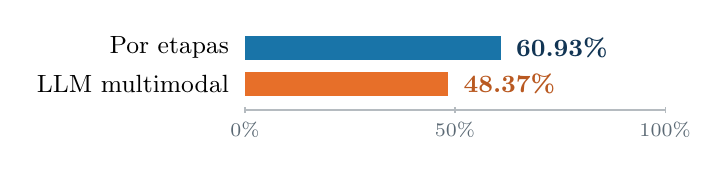
\begin{tikzpicture}[x=0.044\linewidth,y=1.45em]
      \draw[muted!45,line width=0.7pt] (0,0) -- (10,0);
      \foreach \x in {0,5,10}{
        \draw[muted!45] (\x,-0.08) -- (\x,0.08);
        \node[below,font=\scriptsize,text=muted] at (\x,-0.05) {\pgfmathparse{int(\x*10)}\pgfmathresult\%};
      }
      \node[anchor=east,font=\small] at (-0.15,1.55) {Por etapas};
      \fill[blue] (0,1.25) rectangle (6.093,1.85);
      \node[anchor=west,font=\small\bfseries,text=navy] at (6.22,1.55) {60.93\%};
      \node[anchor=east,font=\small] at (-0.15,0.65) {LLM multimodal};
      \fill[orange] (0,0.35) rectangle (4.837,0.95);
      \node[anchor=west,font=\small\bfseries,text=orange!80!black] at (4.97,0.65) {48.37\%};
    \end{tikzpicture}

    El sistema especializado superó a Gemini 2.5 Flash por \textbf{12.6 puntos
    porcentuales}; CER: 0.395 frente a 0.591.
  \end{minipage}
}

\headerbox{Errores, conclusiones y siguiente etapa}{name=discussion,column=1,span=2,below=results}{
  \begin{minipage}[t]{0.26\linewidth}
    \vspace{0pt}
    \centering
    \includegraphics[width=0.92\linewidth,trim=0 910 0 0,clip]{ejemplos_limpieza.png}

    \scriptsize\textcolor{muted}{Dos recortes antes y después de la limpieza de
    bordes y separadores.}
  \end{minipage}\hfill
  \begin{minipage}[t]{0.34\linewidth}
    \vspace{0pt}
    \textbf{Análisis de errores}
    \begin{itemize}\compresslist
      \item dígitos delgados no detectados;
      \item trazos sobre separadores eliminados;
      \item confusiones 8/18 y 7/9;
      \item dificultad en campos con varias casillas.
    \end{itemize}
    Los fallos restantes se concentran en el reconocimiento, no en la ubicación
    de campos. La calidad del escaneo y la caligrafía explican gran parte de la
    variabilidad entre actas.
  \end{minipage}\hfill
  \begin{minipage}[t]{0.36\linewidth}
    \vspace{0pt}
    \textbf{Conclusión científica}

    Separar primero actas digitales y manuscritas es decisivo. En escaneos, la
    alineación con marcas mejora el recorte, mientras que un OCR especializado
    por celdas supera a un LLM multimodal de propósito general.

    \textbf{Siguiente etapa.} Entrenar un reconocedor transformer con pares
    campo-valor del propio dominio; generar etiquetas para YOLOv11 o RT-DETR con
    la plantilla alineada; y evaluar métodos integrales como OmniParser o Donut
    con revisión humana.
  \end{minipage}
}

\end{poster}
\end{document}
